\subsection{Linear Feedback}
%
One of the most common way to calculate corrections is using the following simple formula
%
\begin{align}
\bm{\Delta o_{\text{desired}}} = \bm{M} \bm{\Delta s_{\text{needed}}} 
\label{eq:linearSystemSimple}
\end{align}
%
where $\bm{\Delta o_{\text{desired}}}$ is a vector of the desired variation of a set of
\emph{observables}, which are known to be linearly dependent on the variation of a set of
\emph{correctors}, $\bm{\Delta s_{\text{needed}}}$.
The matrix $\bm{M}$ contains linear coefficients that link observables and correctors. 

Because there were multiple quantities that were corrected using the same algorithm a generic 
library called  \emph{linearFeedback} was developed.
It was implemented as a MATLAB class capable to correct any \emph{observable} parameter available in 
the CERN control system (i.e. reachable via JAPC \cite{Baggiolini:2005}) that 
linearly (or quasi-linearly) responds to the excitation of some
\emph{corrector} that is reachable via the CERN control system.
There is no need to know the linear response between observable and correctors: \emph{linearFeedback} is
able to measure that by exciting the specified correctors and by measuring the response of the
observables.
The natural use of this tool, which also triggered its development, is the beam orbit steering.
Here the beam orbit (observable) is steered by actioning on dipole correctors (steerers).
Often the response matrix is known by the optics model of the line, but there might be issues and
errors that make it interesting, if not necessary, to measure the response matrix on the live machine.
In the following paragraph the main mathematical details of the implementation are presented, followed
by some details of the state of the art of the interface and its use.


\subsubsection{Details of the linearFeedback implementation}
\label{sub:detailLinearFeedback}

Per se the problem is trivial and it only requires to invert the matrix $\bm{M}$. 
The challenge appears when the components of Eq.~\ref{eq:linearSystemSimple} are not well defined, for
example:
%
\begin{itemize}
\item The observables have measurements errors\footnote{In the current implementation of
\emph{linearFeedback} the assumption is made that the steerers are well known and controllable, i.e.
the error in measuring the state $\bm{s_0}$ of the steerers, at any time, is negligible.}.
\item The system is either over-determined (more independent observables than steerers) or
under-determined (more independent steerers than observables).
\item There are hardware limitations on the possible settings of the steerers.
\item %Even if is known a linear relation, 
The elements of the matrix $ \bm{M}$ are not explicitly known.
\item The linearity of the response is ensured only for a sub-space of the correctors/observables spaces.
\end{itemize}
%
The implementation of \emph{linearFeedback} tries to overcome the listed limitations by simple precautions.
The system is always made over-determined: the problem is extended such that the feedback tries not
only to find the steerer settings that produce the wanted observation, 
but also such that the new settings are not \emph{too} far from a desired configuration.
Moreover independent weights can be specified for each of the observables.
These could be specified as inversely proportional to the error in measuring the particular
observable, or according to the user experience or needs.
Equation~\ref{eq:linearSystemSimple} has to be rewritten as:
%
\begin{equation}
\bm{W}
\begin{bmatrix}
\bm{\Delta o_{\text{desired}}}\\
\bm{\Delta s_{\text{desired}}}
\end{bmatrix}
=
\bm{W}
\begin{bmatrix}
\bm{M} \\
\mathds{1}
\end{bmatrix}
\bm{\Delta s_{\text{needed}}}
\label{eq:linearSystemWithDump}
\end{equation}
%
where $\mathds{1}$ is the identity matrix of the appropriate size, $\bm{\Delta
s_{\text{desired}}}$ is the desired variation of the steerer settings, eventually zero, and
$\bm{W}$ is the weight diagonal matrix.
The solution of such a system in a \emph{least-squares} sense is well known \cite{lawson1995solving}:
%
\begin{equation}
\bm{\Delta s_{\text{needed}}} =
\left(
\begin{bmatrix}
\bm{M} \\
\mathds{1}
\end{bmatrix}^T
\bm{W}
\begin{bmatrix}
\bm{M} \\
\mathds{1}
\end{bmatrix}
\right)^{-1}
\begin{bmatrix}
\bm{M} \\
\mathds{1}
\end{bmatrix}^T
\bm{W}
\begin{bmatrix}
\bm{\Delta o_{\text{desired}}}\\
\bm{\Delta s_{\text{desired}}}
\end{bmatrix}
\label{eq:linearSystemWithDumpSolution}
\end{equation}
%
such that the solution minimises the euclidean norm of the weighted residuals:
%
\begin{equation}
\bm{\Delta s_{\text{needed}}} = \bm{x} :\, \min_{\bm{x}} \norm{\bm{W}^{1/2} \left( 
\begin{bmatrix}
\bm{\Delta o_{\text{desired}}}\\
\bm{\Delta s_{\text{desired}}}
\end{bmatrix}  - 
\begin{bmatrix}
\bm{M} \\
\mathds{1}
\end{bmatrix}
\bm{x}
\right)}^2.
\end{equation}
%

The actual implementation of \emph{linearFeedback} does not make use of the solution provided by
Eq.~\ref{eq:linearSystemWithDumpSolution}.
Instead the MATLAB \emph{lsqlin} function \cite{lsqlin} is used. This allows one to specify boundary
conditions on the strength of the available steerers.
The details of the implementation of this function are outside of the scope of this thesis.
The use of the \emph{lsqlin} function has been initially introduced by the attempt to constrain the
steerers not only within their hardware limitation,
but also to give the user the possibility of constraining the strength of each steerer, and eventually
force the system not to move some of the steerers. 
An alternative approach to obtain a similar result is to operate a Singular Value Decomposition (SVD)
of the matrix $\bm{M}$, and apply a cut-off on its singular values.
In the literature (e.g. \cite{Chung:901051}) one can find many different ways to choose the SVD
cut-off, but one has to make some assumption on the system under correction.
From experience at CTF3 it turned out that the most generic approach is still to add tuneable weights,
by means of the matrix $\bm{W}$, to the desired correction ($\bm{\Delta s_{\text{desired}}}$).
A similar approach was also applied in \cite{Latina:2014jca, Latina:2014ama}.

The \emph{linearFeedback} implementation also allows one to compute and see the strength of the
correction and its effect on the observables before applying it.
This allows the user to adjust as desired the weights of observables and steerers before taking any
real action.
Only when the proposed correction and its effect are satisfactory, can the user then apply the
correction with a given gain to (hopefully) approach the solution.
The use of the \emph{lsqlin} function has been preserved for flexibility, but if the steerer weights
are sufficiently large the proposed correction can be made always within the desired steerers limits.

In order to address the case where no trustworthy information is available about the matrix
$\bm{M}$, the \emph{linearFeedback} implements system identification techniques. 
The procedure used to measure the response matrix can be derived from Eq.~\ref{eq:linearSystemSimple}:
%
\begin{align}
\bm{M}  &=
\begin{bmatrix}
\bm{\Delta s_1} & \bm{\Delta s_2} & \cdots &  \bm{\Delta s_n}
\end{bmatrix}^{-1} 
\begin{bmatrix}
\bm{\Delta o_1} & \bm{\Delta o_2} & \cdots &  \bm{\Delta o_n}
\end{bmatrix}
\label{eq:simplestSystemIdentification}
\end{align}
where $\bm{\Delta s_i}$ are a complete set of experimental settings that span the whole linear
space of the steerers, while $\bm{\Delta o_i}$ are the measured variations obtained on the
observables.
%
In the \emph{linearFeedback} different strategies to probe the full space of the steerer settings are
implemented:
\begin{itemize}
\item
Excite each single steerer one after the other.
This is equivalent to measuring one by one the columns of matrix $\bm{M}$.
\item
Randomly (or quasi-randomly) add some controlled noise to the steerers.
\item
Knowing an approximate version of the response matrix $\bm{M}$, apply an excitation to the
steerers such that a desired variation of the observables is performed (e.g. local bumps).
\end{itemize}
The first method is of course the cleanest. However in some cases it is more interesting or necessary
to excite many steerers at the same time.
The last method is instead the best choice for a final tuning of the response matrix and to update it
in case of slow non-linear drifts of the system.
In the implementation of \emph{linearFeedback} the user can choose the most suitable technique.
Moreover, while performing an actual correction, one can decide to use the outcome of each correction
step to keep the response matrix up-to date.
In this case a selectable gain can be used to tune how fast the matrix $\bm{M}$ is updated if the
outcome of a correction is far from the prediction.


\subsubsection{linearFeedback interface and use}
\label{sub:interfaceLinearFeedback}
%
A priori the \emph{linearFeedback} does not need a Graphical User Interface (GUI), but this turned out
to be necessary for daily operations as well as for machine development.
A considerable amount of time has been invested in the development a general purpose GUI, with the
possibility to quickly analyse the data history via the same interface.
The developed GUI is illustrated in Figure~\ref{fig:linearFeedbackGUI}.
%%%%%%%%%%%%%%%%%
\begin{sidewaysfigure}
\centering
\begin{tikzpicture}
    \node[anchor=south west,inner sep=0] (image) at (0,0) {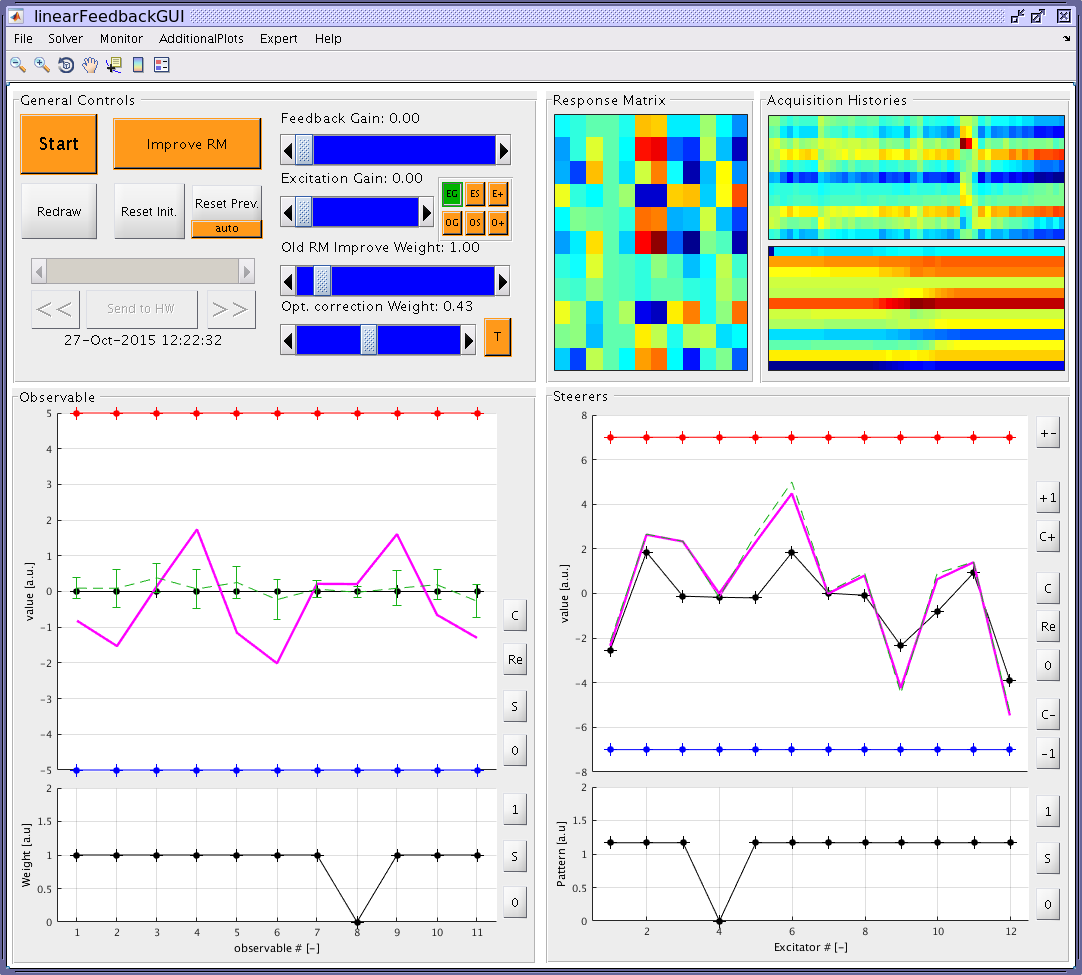
\includegraphics[width=0.55\textwidth]{newFeedbackInterface.png}};
    \begin{scope}[x={(image.south east)},y={(image.north west)}]
    %
    % top top left controls
       \draw[orange,ultra thick,rounded corners, fill=red!20, fill opacity=0.3] (0.01,0.915) rectangle (0.34, 0.975);
       \draw[orange,ultra thick,->] (0.01,0.945) -- (-0.03,0.945) node [left, black, align=right, text width=5cm]  {Advanced menu.};
    % top left controls
        \draw[orange,ultra thick,rounded corners, fill=red!20, fill opacity=0.3] (0.01,0.61) rectangle (0.495, 0.905);
        \draw[orange,ultra thick,->] (0.01,0.75) -- (-0.03,0.75) node [left, black, align=right, text width=5cm] 
        {Main control and parameters for the application. Most important are the feedback gains for correction and response measurement.};
        % top right right
        \draw[orange,ultra thick,rounded corners, fill=red!20, fill opacity=0.3] (0.7,0.61) rectangle (0.99, 0.905);
        \draw[orange,ultra thick,->] (0.99,0.78) -- (1.03,0.78) node [right, black, align=left, text width=5cm] 
        {History of observable acquisitions and steerer settings.};
        % top right
        \draw[orange,ultra thick,rounded corners, fill=red!20, fill opacity=0.3] (0.505,0.61) rectangle (0.69, 0.905);
        \draw[orange,ultra thick,->] (0.69,0.85) -- (1.03,0.93) node [right, black, align=left, text width=5cm] 
        {Response matrix visualisation.};
        % left
        \draw[orange,ultra thick,rounded corners, fill=red!20, fill opacity=0.3] (0.01,0.2) rectangle (0.495, 0.6);
        \draw[orange,ultra thick,->] ((0.01,0.395) -- (-0.03,0.395) node [left, black, align=right, text width=5cm] 
        {Observable acquisition and settings. Red and blue are the tolerated limits for any action. Black is the target reading, magenta is the current reading and dashed-light green is the expected reading after the proposed correction.};
        % right
        \draw[orange,ultra thick,rounded corners, fill=red!20, fill opacity=0.3] (0.505,0.2) rectangle (0.99, 0.6);
        \draw[orange,ultra thick,->] (0.99,0.45) -- (1.03,0.45) node [right, black, align=left, text width=5cm] 
        {Steerer settings. By analogy with the observables view, red and blue are the steerer limits, magenta are the current settings, black the \emph{preferred} or nominal settings, dashed-light green is the proposed correction to achieve the desired observation.};
        % bottom right
        \draw[orange,ultra thick,rounded corners, fill=red!20, fill opacity=0.3] (0.505,0.01) rectangle (0.99, 0.19);
        \draw[orange,ultra thick,->] (0.99,0.1) -- (1.03,0.1) node [right, black, align=left, text width=5cm] 
        {Excitation pattern for the steerers. Eventually used to measure the response matrix between steerers and observables.};
        % bottom left
        \draw[orange,ultra thick,rounded corners, fill=red!20, fill opacity=0.3] (0.01,0.01) rectangle (0.495, 0.19);
        \draw[orange,ultra thick,->] (0.01,0.1) -- (-0.03,0.1) node [left, black, align=right, text width=5cm] 
        {Weight on each observable for computing the correction.};
    \end{scope}
\end{tikzpicture}
\caption{linearFeedback main graphical interface.}
\label{fig:linearFeedbackGUI}
\end{sidewaysfigure}
%
%%%%%%%%%%%%%%%%%
%
This single interface has all the information needed and the means to set-up efficiently the feedback
and control its operation.
Other \emph{expert} settings and diagnostic tools are hidden behind the top main menu.


The \emph{linearFeedback} is by itself a library, and not a tool usable out of the box,
but it provides a generic framework that can be applied to nearly any linear system.
\emph{LinearFeedback} also takes care of the interface with the CERN control system via the developed
MATLAB/JAPC library described in Section~\ref{s:dataacq}.
To be practically usable one needs only to implement a function to translate the signals coming from
the CERN infrastructures into proper observables and settings,
and a function to translate the steerer settings suggested by the feedback to proper commands
understandable by the steerer hardware.
What triggered the development of such infrastructure was the necessity to have an easy and flexible
way to keep under control orbits and dispersion in the DBRC.
For this specific use an additional \emph{orbitCorrection} tool has been implemented.
\emph{OrbitCorrection} is just a specialised ``MATLAB subclass'' of \emph{linearFeedback}. Its main
task is to implement the concept of beam orbit and dispersion as observables, 
and a function to directly act on the dipole correctors installed in the CTF3 beamlines.
For further flexibility the  \emph{orbitCorrection} was compiled as a standalone application that
requires an XML configuration file.
This is user-editable, and it contains mainly the signals of the BPMs to use as simple orbit or as
dispersion measurement points, and the list of corrector magnets.
The ``beam dispersion'' definition implemented in the \emph{orbitCorrection} tool is a linear fit of
the beam jitter at each BPM location with respect to a reference BPM where the dispersion is assumed
to be known and constant.
This turned out to be the most reliable and generic dispersion measurement of the ones described in
Section~\ref{s:dispersiontool}.

The \emph{orbitCorrection} is only an example of use of the \emph{linearFeedback} library.
The use of \emph{linearFeedback} has been applied also to solve different problems than the orbit
steering. Some of these results will be presented in Section~\ref{s:otherApplications}.
%Further details on the implementation are outside the scope of this work, 










